% -*- coding: utf-8 -*-
\documentclass[12pt]{article}
\usepackage{errc2007-xenvsopenvz}

\usepackage{graphicx,url}

\usepackage[portuges]{babel}
%\usepackage{ucs}
\usepackage[utf8x]{inputenc} 

\usepackage{xspace}
\def\sw{\textit{software}\xspace}
\def\hw{\textit{hardware}\xspace}
\def\hvisor{\textit{hypervisor}\xspace}
     
\sloppy

\title{Análise de Desempenho da Virtualização de Rede nos Sistemas Xen e OpenVZ}

\author{Adler Hoff Schmidt\inst{2}, Márcio Parise Boufleur\inst{1}, Ronaldo Canofre M. dos Santos\inst{2},\\ Andrea Schwertner Charão\inst{1},\inst{2}}

\address{Laboratório de Sistemas de Computação (LSC)
  \nextinstitute
  Programa de Educação Tutorial (PET)\\
  Curso de Ciência da Computação -- Universidade Federal de Santa Maria (UFSM)\\
  Campus UFSM -- 97105-900 -- Santa Maria -- RS -- Brasil
  \email{\{adlerhs,boufleur,canofre,andrea\}@inf.ufsm.br}
}

\begin{document} 

\maketitle

% Na chamada da ERRC207 diz que abstract não é necessário
%\begin{abstract}
%\end{abstract}

% Na primeira versão do resumo faltava uma maior ênfase em redes. (andrea)   
\begin{resumo} 
Tecnologias de virtualização vêm sendo amplamente utilizadas em sistemas interligados em rede. Existem diferentes abordagens e ferramentas para o suporte a múltiplas máquinas virtuais compartilhando os recursos físicos de um sistema hospedeiro. Neste trabalho, analisa-se o desempenho de rede dos sistemas Xen e OpenVZ, que seguem diferentes abordagens e constituem duas soluções populares de virtualização. O foco no desempenho de rede justifica-se porque muitos sistemas virtualizados executam serviços e aplicações que necessitam de comunicação pela rede. Para investigar o impacto da virtualização no desempenho de rede, utilizou-se um benchmark clássico em um mesmo sistema, com e sem o uso de virtualização.
\end{resumo}

% A frase abaixo não me parecia tão importante para ser colocada num resumo. (andrea) 
%Existem quatro métodos de virtualização conhecidos: emulação, virtualização nativa, paravirtualização e virtualização em nível do sistema operacional. 
%Desses quatro, decidimos selecionar os dois últimos citados, que são mais usados, e testar seu desempenho na transferência de arquivos em uma rede. Usamos o Xen representando a paravirtualização e o OpenVZ representando o outro método. 
%E então propormos a comparação entre esses dois e também com as máquinas sem virtualização alguma.

\section{Introdução}
%\begin{itemize}
%\item Virtualização é um tema atual
%\item Há diversas soluções de virtualização em nível de SO
%\item Dentre os fatores a considerar na escolha de uma solução, tem-se o desempenho da rede
%\item Xen e OpenVZ tem sido comparados ultimamente. Neste artigo, o foco é a virtualização da rede nesses sistemas.
%\end{itemize}
%-----------------------------------------------------------------------------

Atualmente, a virtualização em ambientes computacionais constitui um tema de pesquisa e desenvolvimento que permeia várias áreas da computação. A capacidade de multiplexação de diversos sistemas operacionais sobre um mesmo \hw permite um aproveitamento mais racional dos recursos disponíveis, provendo economia, flexibilidade, segurança, gerenciabilidade de sistemas de \sw e um bom isolamento de falhas.

Diversos métodos e ferramentas de virtualização têm sido propostos, tornando pouco trivial a escolha de uma solução que atenda aos requisitos de cada ambiente. Dentre os fatores a considerar, o desempenho de rede é um crucial, uma vez que os sistemas atuais dependem fortemente de comunicação entre si. 

Dentre as soluções de virtualização disponíveis atualmente no mercado, VMware~\cite{vmware}, Xen~\cite{xen} e OpenVZ~\cite{openvz} vêm ganhando atenção considerável. De fato, estes sistemas são expoentes de abordagens de virtualização populares, sendo o primeiro uma solução proprietária e os demais soluções livres que têm sido extensivamente comparados ultimamente~\cite{xenvsopenvz}, sendo que Xen já foi alvo de avaliações de desempenho~\cite{urschei2007amorvm}. Neste trabalho, tem-se como objetivo analisar o desempenho da rede em sistemas que usam Xen ou OpenVZ. Para avaliar o desempenho das soluções, optou-se por utilizar o \emph{benchmark} de rede Netperf~\cite{netperf}. Esta ferramenta de análise de desempenho foi escolhida por sua capacidade de análise sintética de resultados e pela grande quantidade de outros estudos que utilizaram a mesma. Assim, compararemos os resultados obtidos em um mesmo ambiente, com e sem a utilização das soluções de virtualização selecionadas.

%Para isso, compara-se os resultados obtidos com o \emph{benchmark} de rede Netperf~\cite{netperf} em um mesmo ambiente, com e sem o uso dessas ferramentas. 

O restante deste artigo está organizado como segue: na seção \ref{s:tecnologias}, expõe-se os conceitos gerais sobre virtualização e as tecnologias existentes, abordando-se as características gerais de Xen e OpenVZ. Na seção \ref{s:virtualizacao}, descreve-se as formas como ambas as tecnologias implementam a virtualização da rede. Na seção \ref{s:desempenho}, apresenta-se a análise de desempenho, que constitui a principal contribuição deste trabalho, detalhando-se a metodologia utilizada e os resultados obtidos. Na seção \ref{s:fim}, por fim, apresenta-se as considerações finais sobre o trabalho.


\section{Tecnologias de Virtualização}\label{s:tecnologias}

Visando o melhor aproveitamento do poder dos \textit{mainframes}, no início da década de 70, foi criada uma técnica para permitir que diversas máquinas virtuais compartilhassem o mesmo \hw subjacente ~\cite{Goldberg}. Basicamente, a virtualização é uma técnica que insere uma camada extra de \sw entre o sistema físico e o sistema operacional. Dessa forma, diversos sistemas operacionais podem executar concorrentemente sobre o mesmo \hw, com a camada extra de \sw, conhecida como Monitor de Máquinas Virtuais (MMV) ou \hvisor, controlando o acesso físico dos mesmos ao \hw. Esta organização clássica de um sistema virtualizado é ilustrada na figura \ref{fig:virtualizacao}.


\begin{figure}[!htb]
\centering
\resizebox{7cm}{!}{\includegraphics{figuras/classica.eps}}
\caption{Estrutura clássica de um sistema virtualizado}
\label{fig:virtualizacao}
\end{figure}


Com o aumento do poder de processamento dos computadores atuais, algumas soluções de virtualização foram implementadas para executar em sistemas de médio e pequeno porte, incluindo computadores pessoais. Dentre essas soluções, Xen~\cite{xen} destaca-se por ser um monitor de máquinas virtuais de código aberto, que provê um alto grau de desacoplamento entre os sistemas hospedados e o \hw abaixo deles.

Atualmente, uma nova técnica de virtualização começou a receber destaque: a virtualização em nível de sistema operacional. Essa técnica difere da técnica clássica por inserir as máquinas virtuais no mesmo nível do \hvisor. Assim, as máquinas virtuais sobre essa arquitetura compartilham o mesmo \emph{kernel} do sistema hospedeiro, o que reduz significativamente a sobrecarga de criação de uma nova máquina virtual. Porém, essa solução possui flexibilidade reduzida, uma vez que só é possível a execução de um sistema operacional hospedado idêntico ao hospedeiro. Um expoente desse método de virtualização é o MMV OpenVZ~\cite{openvz}.

As seções \ref{s:xen} e \ref{s:openvz} apresentam outras características de Xen e OpenVZ que motivaram a escolha destes sistemas para a realização deste trabalho.

% Exemplos de implementação dessa técnica são o OpenVZ~\cite{openvz} e Solaris Zones~\cite{price2004szo}.

%\textbf{Essa frase da introdução deve ficar melhor nessa seção:}
%Dentre os métodos populares atualmente, tem-se a virtualização baseada em hipervisores -- utilizada por exemplo em VMWare~\cite{vmware} e Xen~\cite{xen} -- e a virtualização no nível do sistema operacional -- como OpenVZ~\cite{openvz} e Solaris Zones~\cite{solaris-zones}.

%\begin{itemize}
%\item Introduzir de modo geral os conceitos relacionados a virtualização e as tecnologias existentes
%\item Falar das características gerais de Xen e OpenVZ (uma subseção para cada um)
%\end{itemize}

\subsection{Xen}\label{s:xen}

Xen é um monitor de máquinas virtuais de código aberto, com suporte a diversas arquiteturas, como IA-32, AMD64 e EM64T. Para implementar a virtualização nessas arquiteturas, Xen utiliza-se da técnica de paravirtualização~\cite{youseff2006phs}. Esta técnica consiste em fazer uma pequena modificação dos sistemas operacionais que irão executar, de modo a garantir que os mesmos não sejam executados no mesmo nível do MMV. Apesar da necessidade da modificação do sistema operacional para execução sobre o Xen, esta abordagem é eficiente e não torna necessária a modificação das aplicações do usuário.

Algumas arquiteturas mais recentes possuem extensões de virtualização em nível de processador. Exemplos incluem AMD\textit{Pacifica} e Intel \textit{Virtualization Technology} (VT). Com o uso de tais arquiteturas, sistemas operacionais cujos núcleos não permitem modificação podem executar normalmente sobre o \hvisor Xen.

\subsection{OpenVZ}\label{s:openvz}

OpenVZ é uma tecnologia de virtualização em nível de sistema operacional baseada no sistema GNU/Linux. Nesta abordagem de virtualização, todas as máquinas executam o mesmo núcleo do sistema operacional, o que impõe uma sobrecarga baixa na criação e gerenciamento de máquinas virtuais.

Em OpenVZ, as máquinas virtuais são totalmente isoladas entre si, possuindo arquivos, usuários e grupos, árvores de processos, rede, dispositivos e comunicação entre processos de forma totalmente única e compartimentada. 

Devido ao fato de utilizar virtualização no nível de sistema operacional, OpenVZ suporta apenas sistemas hospedados que sejam compatíveis com o núcleo do hospedeiro. Ou seja, apenas o sistema operacional GNU/Linux pode ser hospedado, mas a distribuição do mesmo não é necessariamente a mesma do hospedeiro.

% uma figurinha ficaria legal aqui.

%-----------------------------------------------------------------------------
\section{Virtualização da Rede em Xen e OpenVZ}\label{s:virtualizacao}

Existem diversos métodos de se implementar uma interface de rede virtualizada. Os sistemas Xen e OpenVZ utilizam abordagens distintas para resolver esta questão.

Em Xen, as interfaces de rede virtuais são implementadas através de páginas de memória compartilhada entre o \hvisor e o sistema operacional hospedado. Este compartilhamento se dá através de anéis de descritores assíncronos, que contêm \emph{buffers} de entrada e saída que são alocados pelo sistema operacional hospedado~\cite{urschei2007amorvm}. Dessa forma, a necessidade de cópias entre o MMV e o sistema hospedado é reduzida. 

Para comunicação entre as máquinas virtuais, Xen implementa uma \emph{bridge} virtual, dispensando assim a necessidade de \emph{broadcast} entre as interfaces virtuais. A figura \ref{fig:xen_net} apresenta a organização da rede virtual de Xen. Nesta figura, uma \emph{bridge} virtual entre a interface física e as interfaces virtualizadas é criada no domínio administrativo (\emph{Driver Domain}), provendo assim conectabilidade entre as máquinas virtuais hospedadas (\emph{Guest Domain}) e a rede externa. A conexão entre os domínios hospedados e o domínio administrativo é feita através de um canal de entrada e saída (\emph{I/O channel}).


\begin{figure}[!htb]
\centering
\resizebox{9cm}{!}{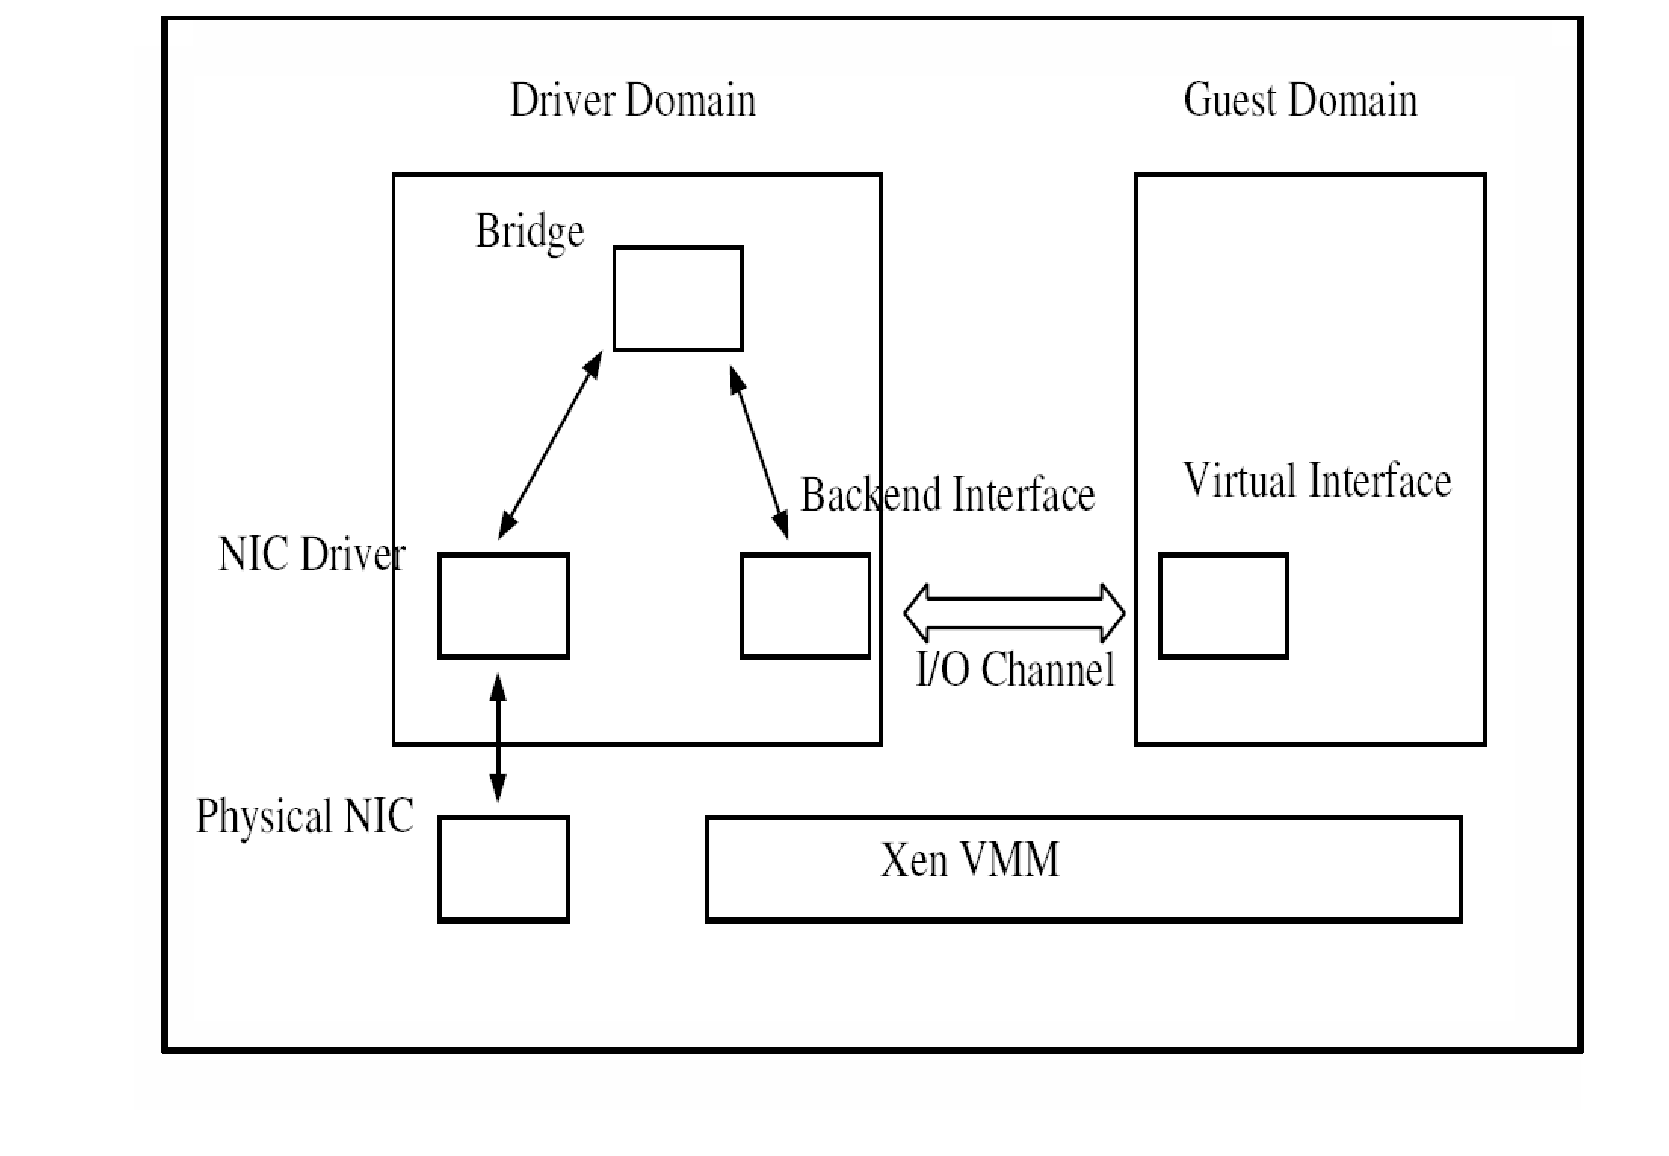
\includegraphics{figuras/xen_net.eps}}
\caption{Estrutura de rede virtual de Xen ~\cite{menon2006onv}}
% A professora não acredita que eu fale chinês :-)
\label{fig:xen_net}
\end{figure}

No que diz respeito a OpenVZ, uma vez que as máquinas virtuais situam-se no mesmo nível do sistema hospedeiro, são criadas interfaces virtuais interligadas com o hospedeiro via uma conexão ponto-a-ponto. Esta abordagem permite que o envio e recebimento de pacotes seja feito pelo módulo de roteamento do núcleo do sistema hospedeiro, fator esse que simplifica a questão da virtualização da rede de OpenVZ~\cite{openvz}.

%Explicar em maiores detalhes como é implementada a virtualização (ou não) da rede nesses sistemas.

\section{Análise de Desempenho}\label{s:desempenho}

%\begin{itemize}
%\item Descrever os objetivos específicos da análise. P.ex.: investigar latência e taxa de transmissão.
%\item Descrever o ambiente de testes (hw + sw). Não esqueçam de usar um cabo cross para ligar diretamente as 2 máquinas. Os resultados serão mais confiáveis assim.
%\item Apresentar os resultados
%\item Discutir os resultados (o que era esperado com base nas características dos 2 sistemas? obteve-se o que era esperado? há diferenças significativas entre os 2 sistemas?)
%\end{itemize}


Os experimentos realizados tinham como principal objetivo analisar o desempenho de rede face ao uso das ferramentas Xen e OpenVZ. Para isso, decidiu-se utilizar o \emph{benchmark} Netperf em um ambiente composto por dois computadores idênticos interconectados. Esse ambiente foi alternadamente configurado de três formas: sem virtualização, com virtualização baseada em Xen e com virtualização baseada em OpenVZ. Nos dois casos com virtualização, utilizou-se apenas uma máquina virtual sobre cada máquina real.

Para a realização dos testes foram utilizados dois computadores com arquitetura Intel x86, Pentium IV com processadores de 2.8GHz e memória de 512M. O sistema operacional adotado para os testes foi Ubuntu Linux 7.04, com \emph{kernel} 2.6.19-4. As versões do Xen e do OpenVZ analisados são respectivamente 3.0.3 e 028stab035.1. A interligação entre as máquinas foi feita através de um \emph{switch} Ethernet de 100 Mbps. Os testes foram realizados em um ambiente controlado, para evitar influência de tráfego adicional na rede.

O \emph{benchmark} Netperf permite medir o desempenho de rede segundo diferentes métricas. Para os experimentos realizados, a métrica escolhida foi a taxa de transferência da rede, analisada através de comunicações Request-Response com os protocolos TCP e UDP. Os testes foram realizados com três grupos de tamanhos de mensagens: mensagens pequenas (até 512 bytes), médias (até 512 Kbytes) e grandes (até 50 Mbytes). Em todos os casos, foram mantidos os valores \emph{default} em Netperf para outros parâmetros da comunicação (por exemplo, \emph{buffer} de sistema e MTU~\cite{netperf}). Para a obtenção dos resultados a seguir foram realizadas 10 execuções para cada tamanho de pacote, sendo calculado para a anáise dos mesmos, a média aritmética, o desvio padrão, o coeficiente de variação e a mediana. 



% Duas máquinas com hardware idênticos: definições do hardware?
% Foram ligadas 
% Mais alguma coisa?


\subsection{Resultados Obtidos}

Os gráficos apresentados a seguir reúnem os resultados obtidos nas medições efetuadas. Todos os gráficos apresentam o tamanho das mensagens no eixo das abscissas e a taxa de transferência no eixo das ordenadas.

Nas figuras \ref{fig:tcp_peq} e \ref{fig:tcp_med} tem-se os resultados obtidos com o protocolo TCP para mensagens de tamanho pequeno e médio, respectivamente. O coeficiente de variação para mensagens pequenas ficou abaixo de 7,89 x 10^{-3} para o Xen, 28,16 x 10^{-3} para OpenVZ e 20,91 x 10^{-3} para máquina sem virtualização. Em mensagens médias esses valores foram de 23,24 x 10^{-3} para Xen,7,59 x 10^{-3} para OpenVZ e 58,57 x10^{-3} nas execuções sem virtualizaçào. Mensagens deste grupo são comuns em serviços básicos de rede. Na figura \ref{fig:tcp_grande} tem-se os resultados para mensagens de tamanho grande, também com o protocolo TCP, onde o maior coeficiente de variação foi de 2,73 x 10^{-1} para Xen e 2.52 x10^{-1} para OpenVZ e execuções sem virtualização. Mensagens deste grupo são típicas em aplicações que exigem transferência de arquivos.

\begin{figure}[!htb]
\centering
\resizebox{9cm}{!}{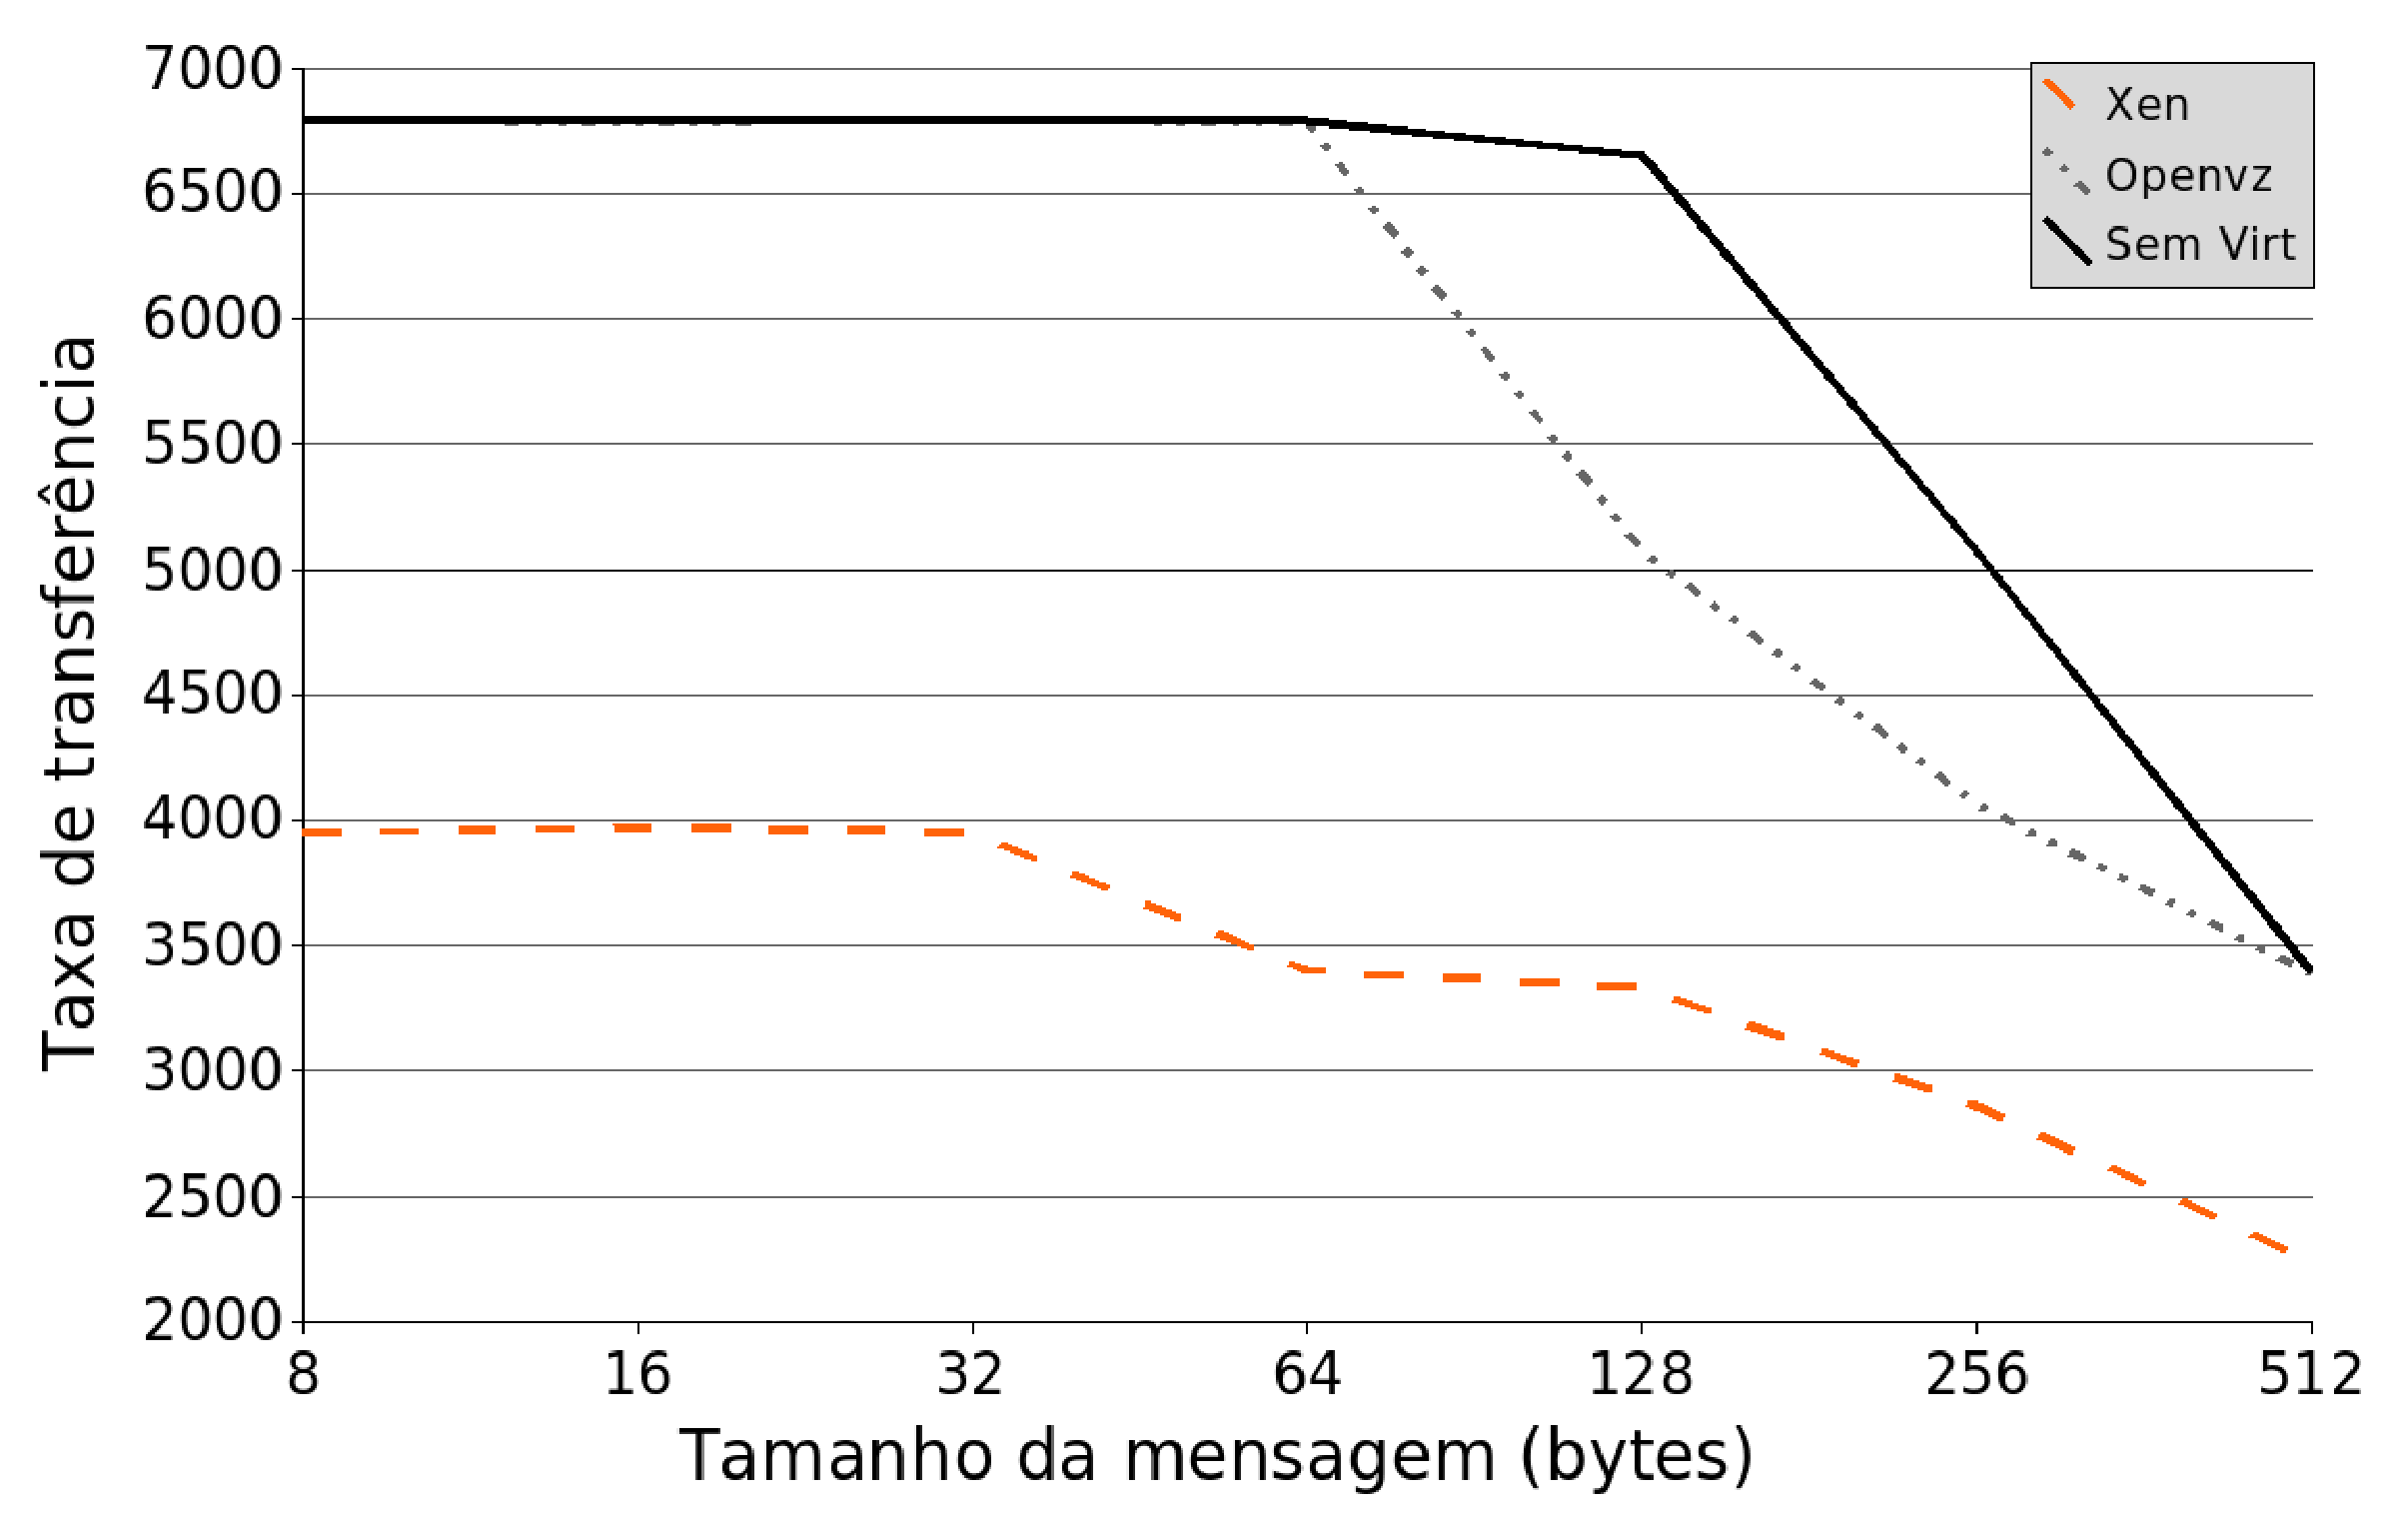
\includegraphics{figuras/tcp_peq.eps}}
\caption{Taxas de transferência TCP, com mensagens pequenas, até 512 bytes}
\label{fig:tcp_peq}
\end{figure}

\begin{figure}[!htb]
\centering
\resizebox{9cm}{!}{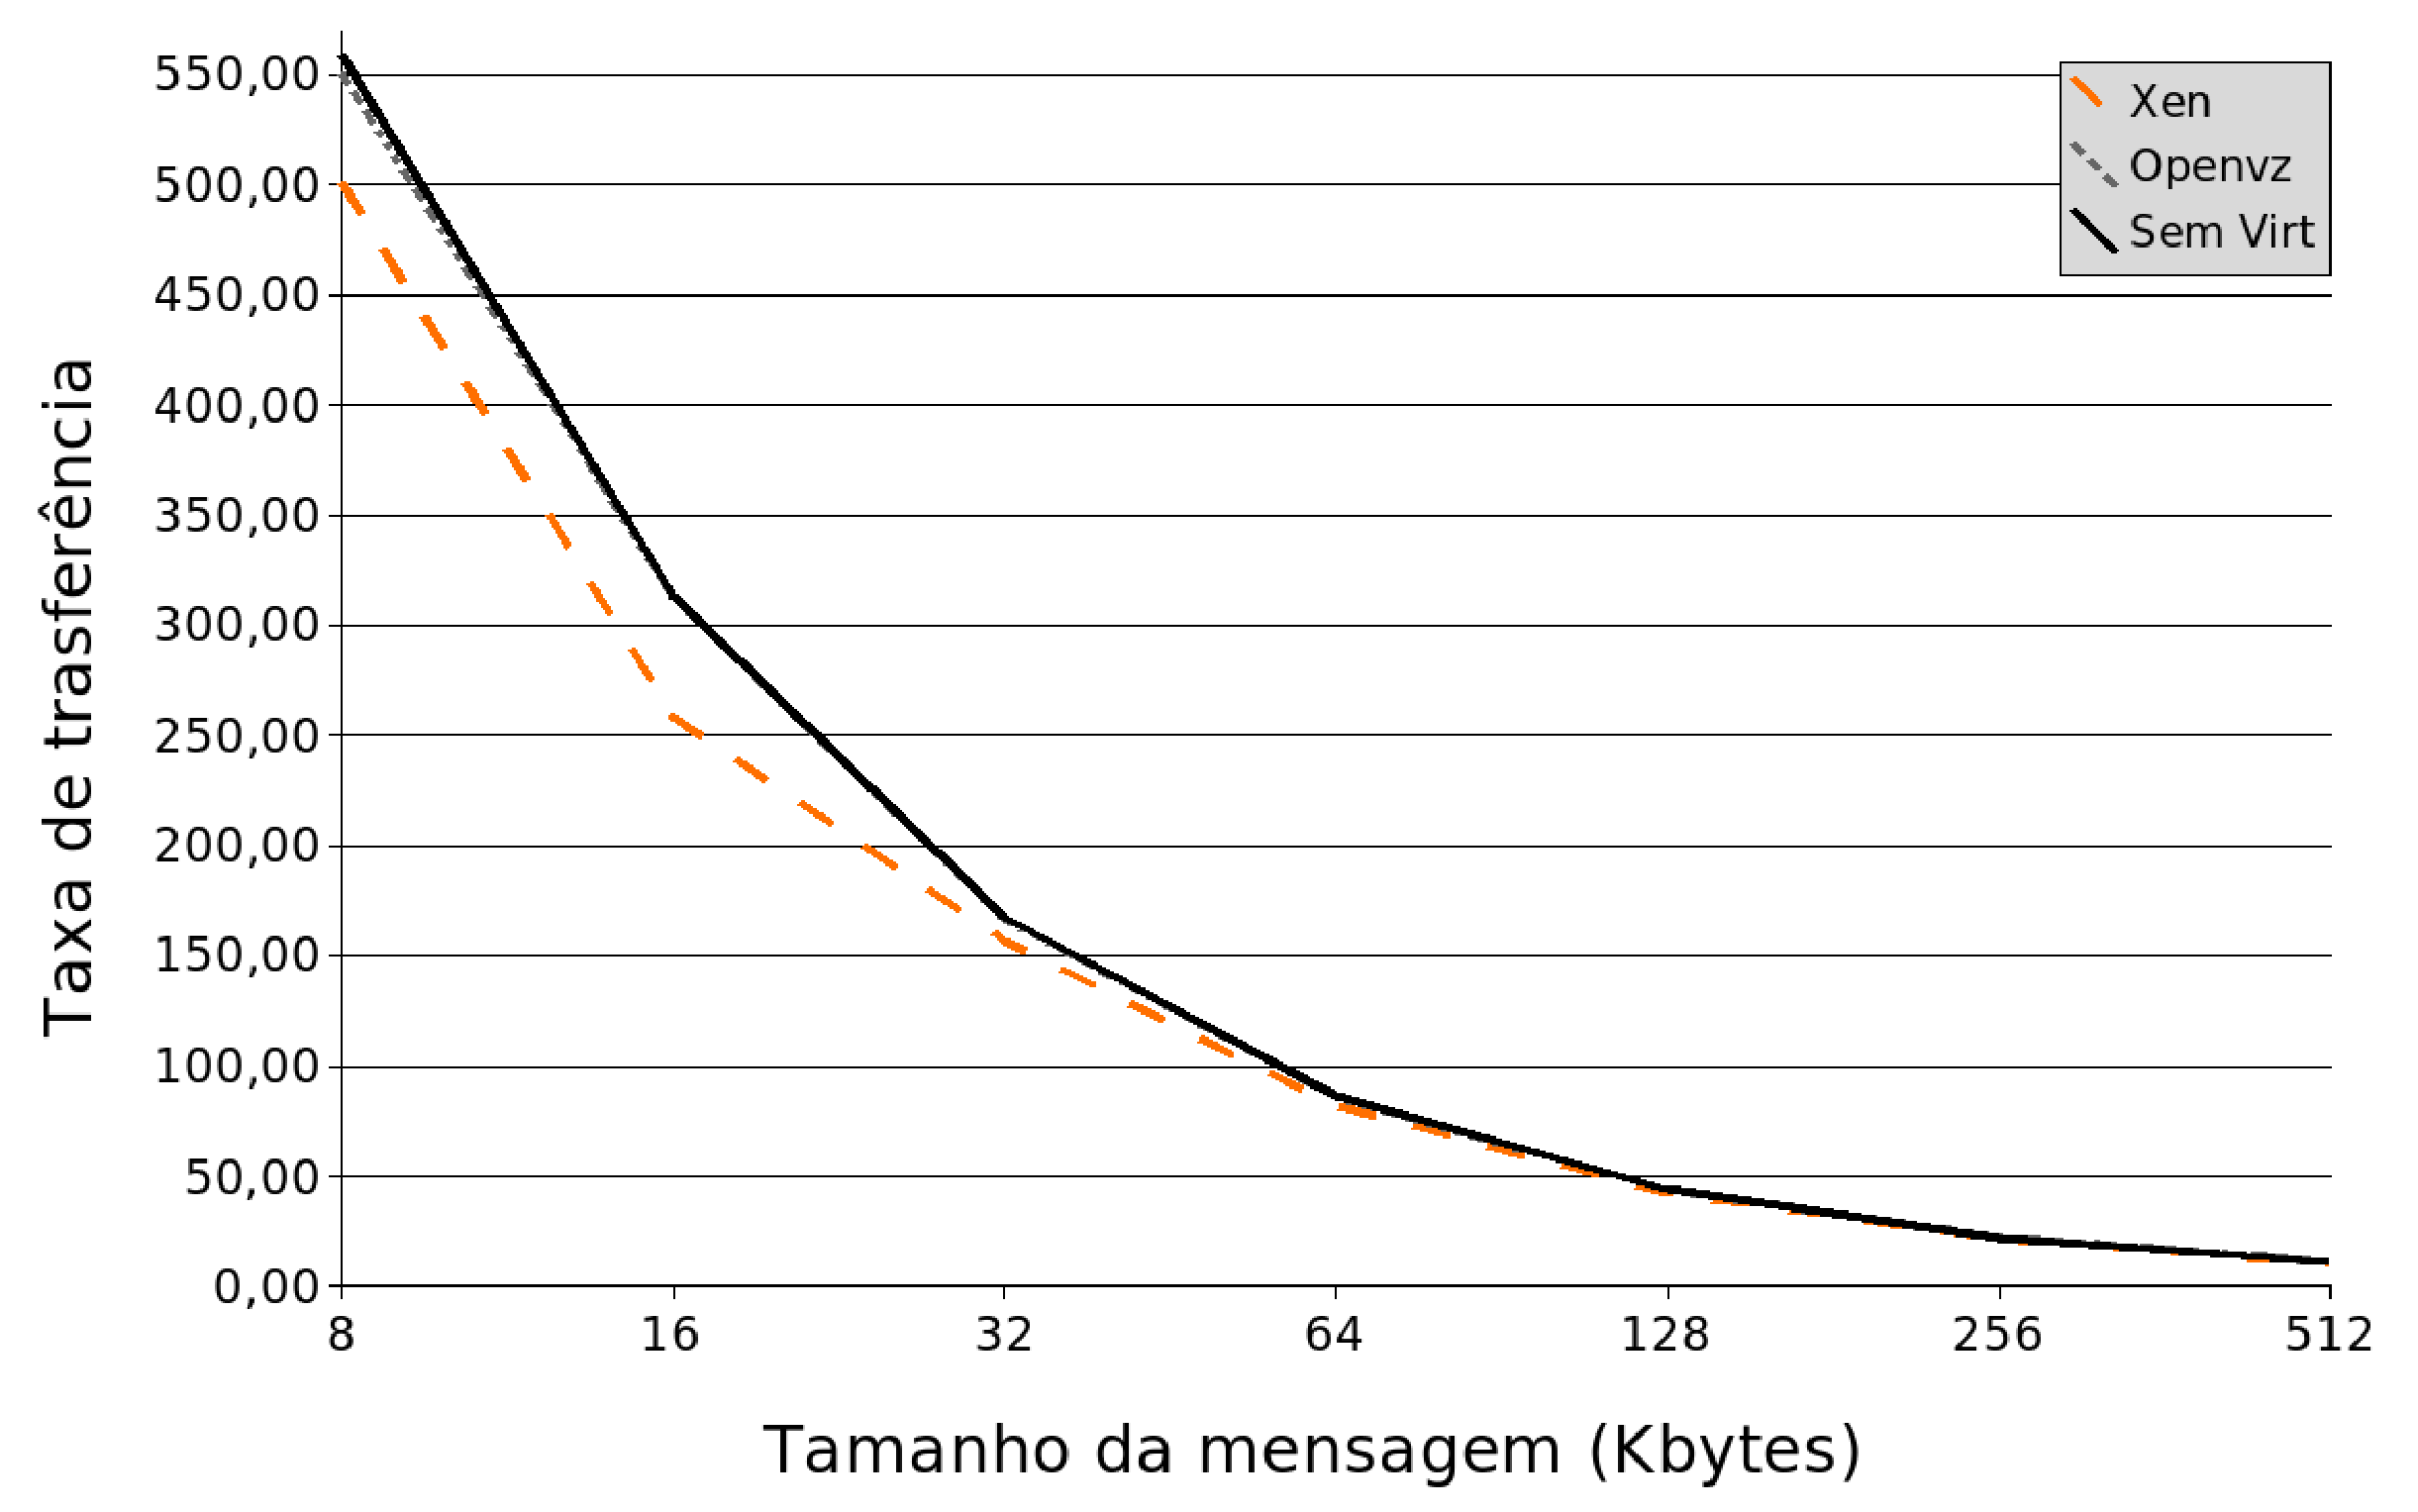
\includegraphics{figuras/tcp_medio.eps}}
\caption{Taxas de transferência TCP, com mensagens de tamanho médio, entre 8 e 512 Kbytes}
\label{fig:tcp_med}
\end{figure}

As figuras \ref{fig:udp_peq} e  \ref{fig:udp_med} apresentam os resultados das medições com o protocolo UDP para mensagens pequenas e médias, respectivamente. Para as mensagnes trasferidas por UDP o coeficiente de variação máximo obitido para mensagens pequenas foi de 15,15 x 10^{-3} no Xen, 24.12 x 10^{-3} no OpenVZ e 88,44 x 10^{-3} em execuções sem virtualização. Nas mensagens médias transferidas por UDP, os valores máximos obitidos foram  e 19,68 x 10^{-3} no Xen, 5.32  x 10^{-3} no OpenVZe 5,39 x 10^{-3} em execuções sem virtualizaçào. Vale ressaltar que devido às restrições do protocolo, o Netperf, por \emph{default} não permite a transmissão de mensagens grandes com UDP.


\subsection{Análise dos Resultados}

Como se pode observar, os gráficos para mensagens pequenas evidenciam diferenças significativas entre as taxas de transferência nas situações analisadas. Esperava-se, de fato, que o desempenho da comunicação entre as máquinas sem virtualização seria melhor do que nos casos com Xen ou OpenVZ. Essa expectativa se concretizou na maior parte dos casos.

Quanto à comparação entre Xen e OpenVZ, o desempenho deste último foi superior ao primeiro, principalmente para mensagens de tamanho pequeno e médio. Isso explica-se pois Xen usa a técnica de paravirtualização, em que são necessárias modificações no \emph{kernel} do sistema operacional hóspede. Já OpenVZ utiliza virtualização no nível do sistema operacional, assim o mesmo \emph{kernel} é usado para executar os ambientes no hospedeiro. Embora este comportamento fosse esperado, notou-se que para certos tamanhos dos pacotes OpenVZ consegue atingir uma taxa de transmissão muito próxima, senão igual, ao caso sem virtualização. Essa constatação é um ponto favorável para a escolha do OpenVZ para sistemas virtualizados em que o desempenho da rede é crítico.

\begin{figure}[!htb]
\centering
\resizebox{9cm}{!}{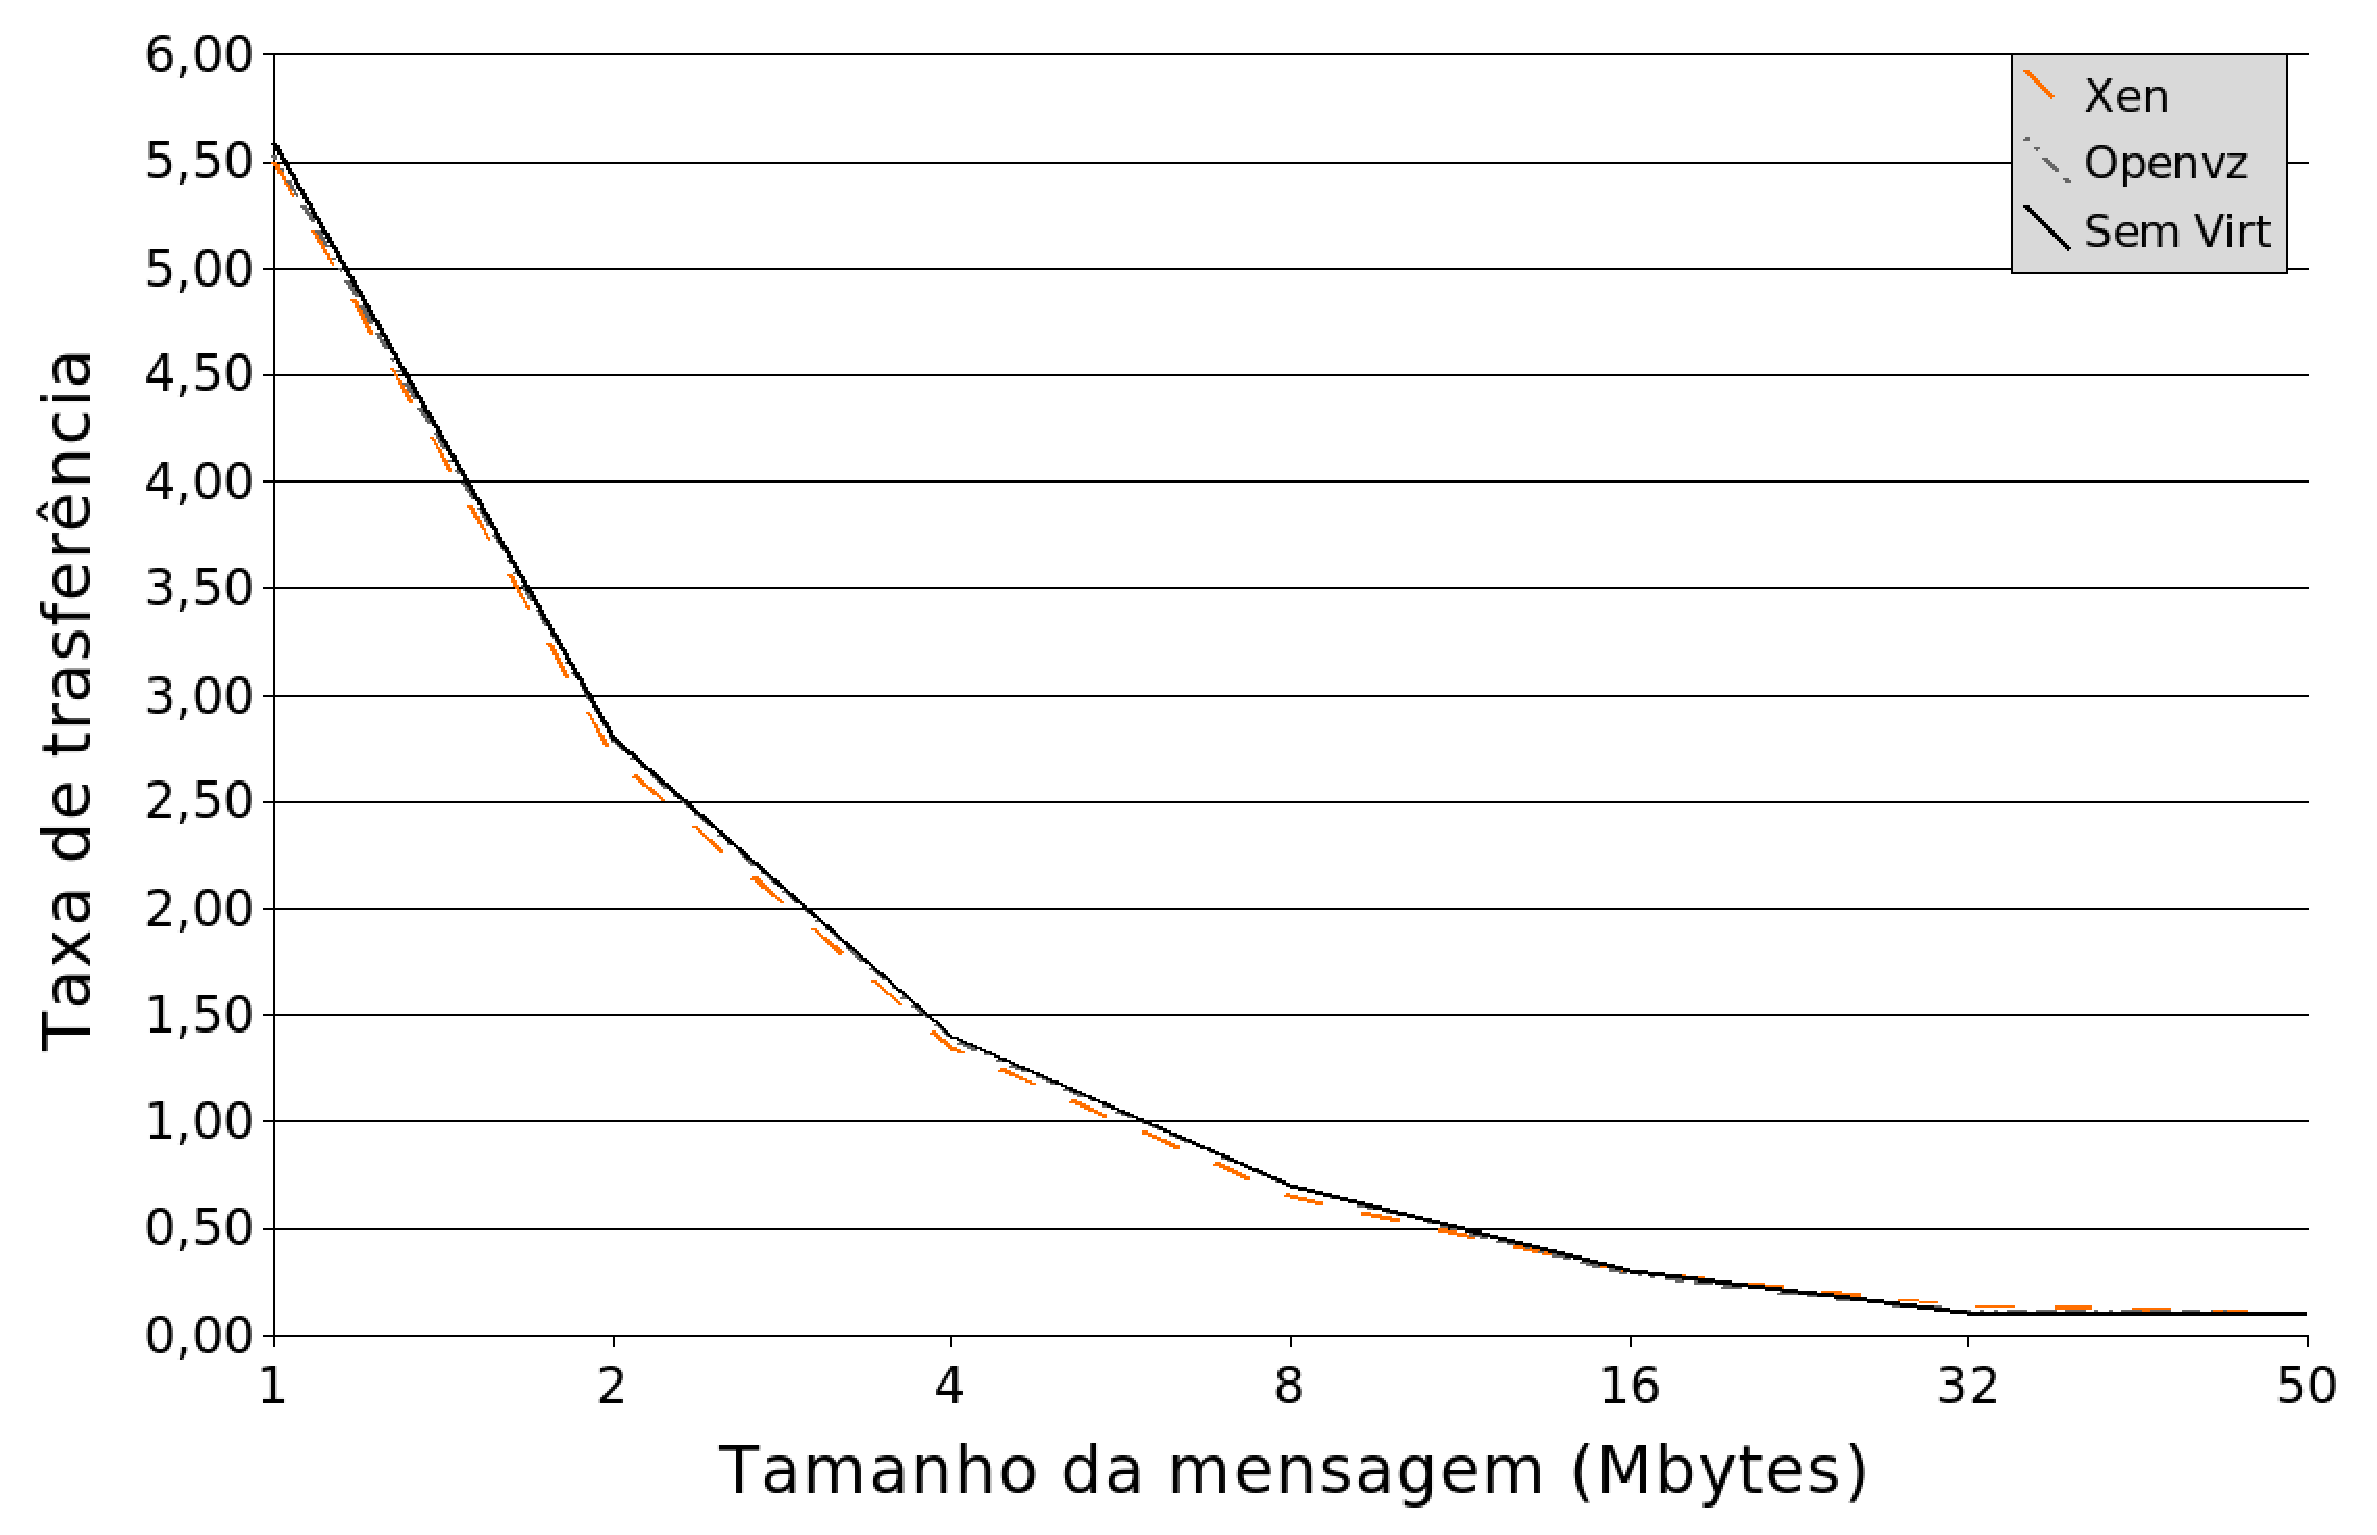
\includegraphics{figuras/tcp_grande.eps}}
\caption{Taxas de transferência TCP, com mensagens grandes, de 1 a 50 Mbytes}
\label{fig:tcp_grande}
\end{figure}

\begin{figure}[!htb]
\centering
\resizebox{9cm}{!}{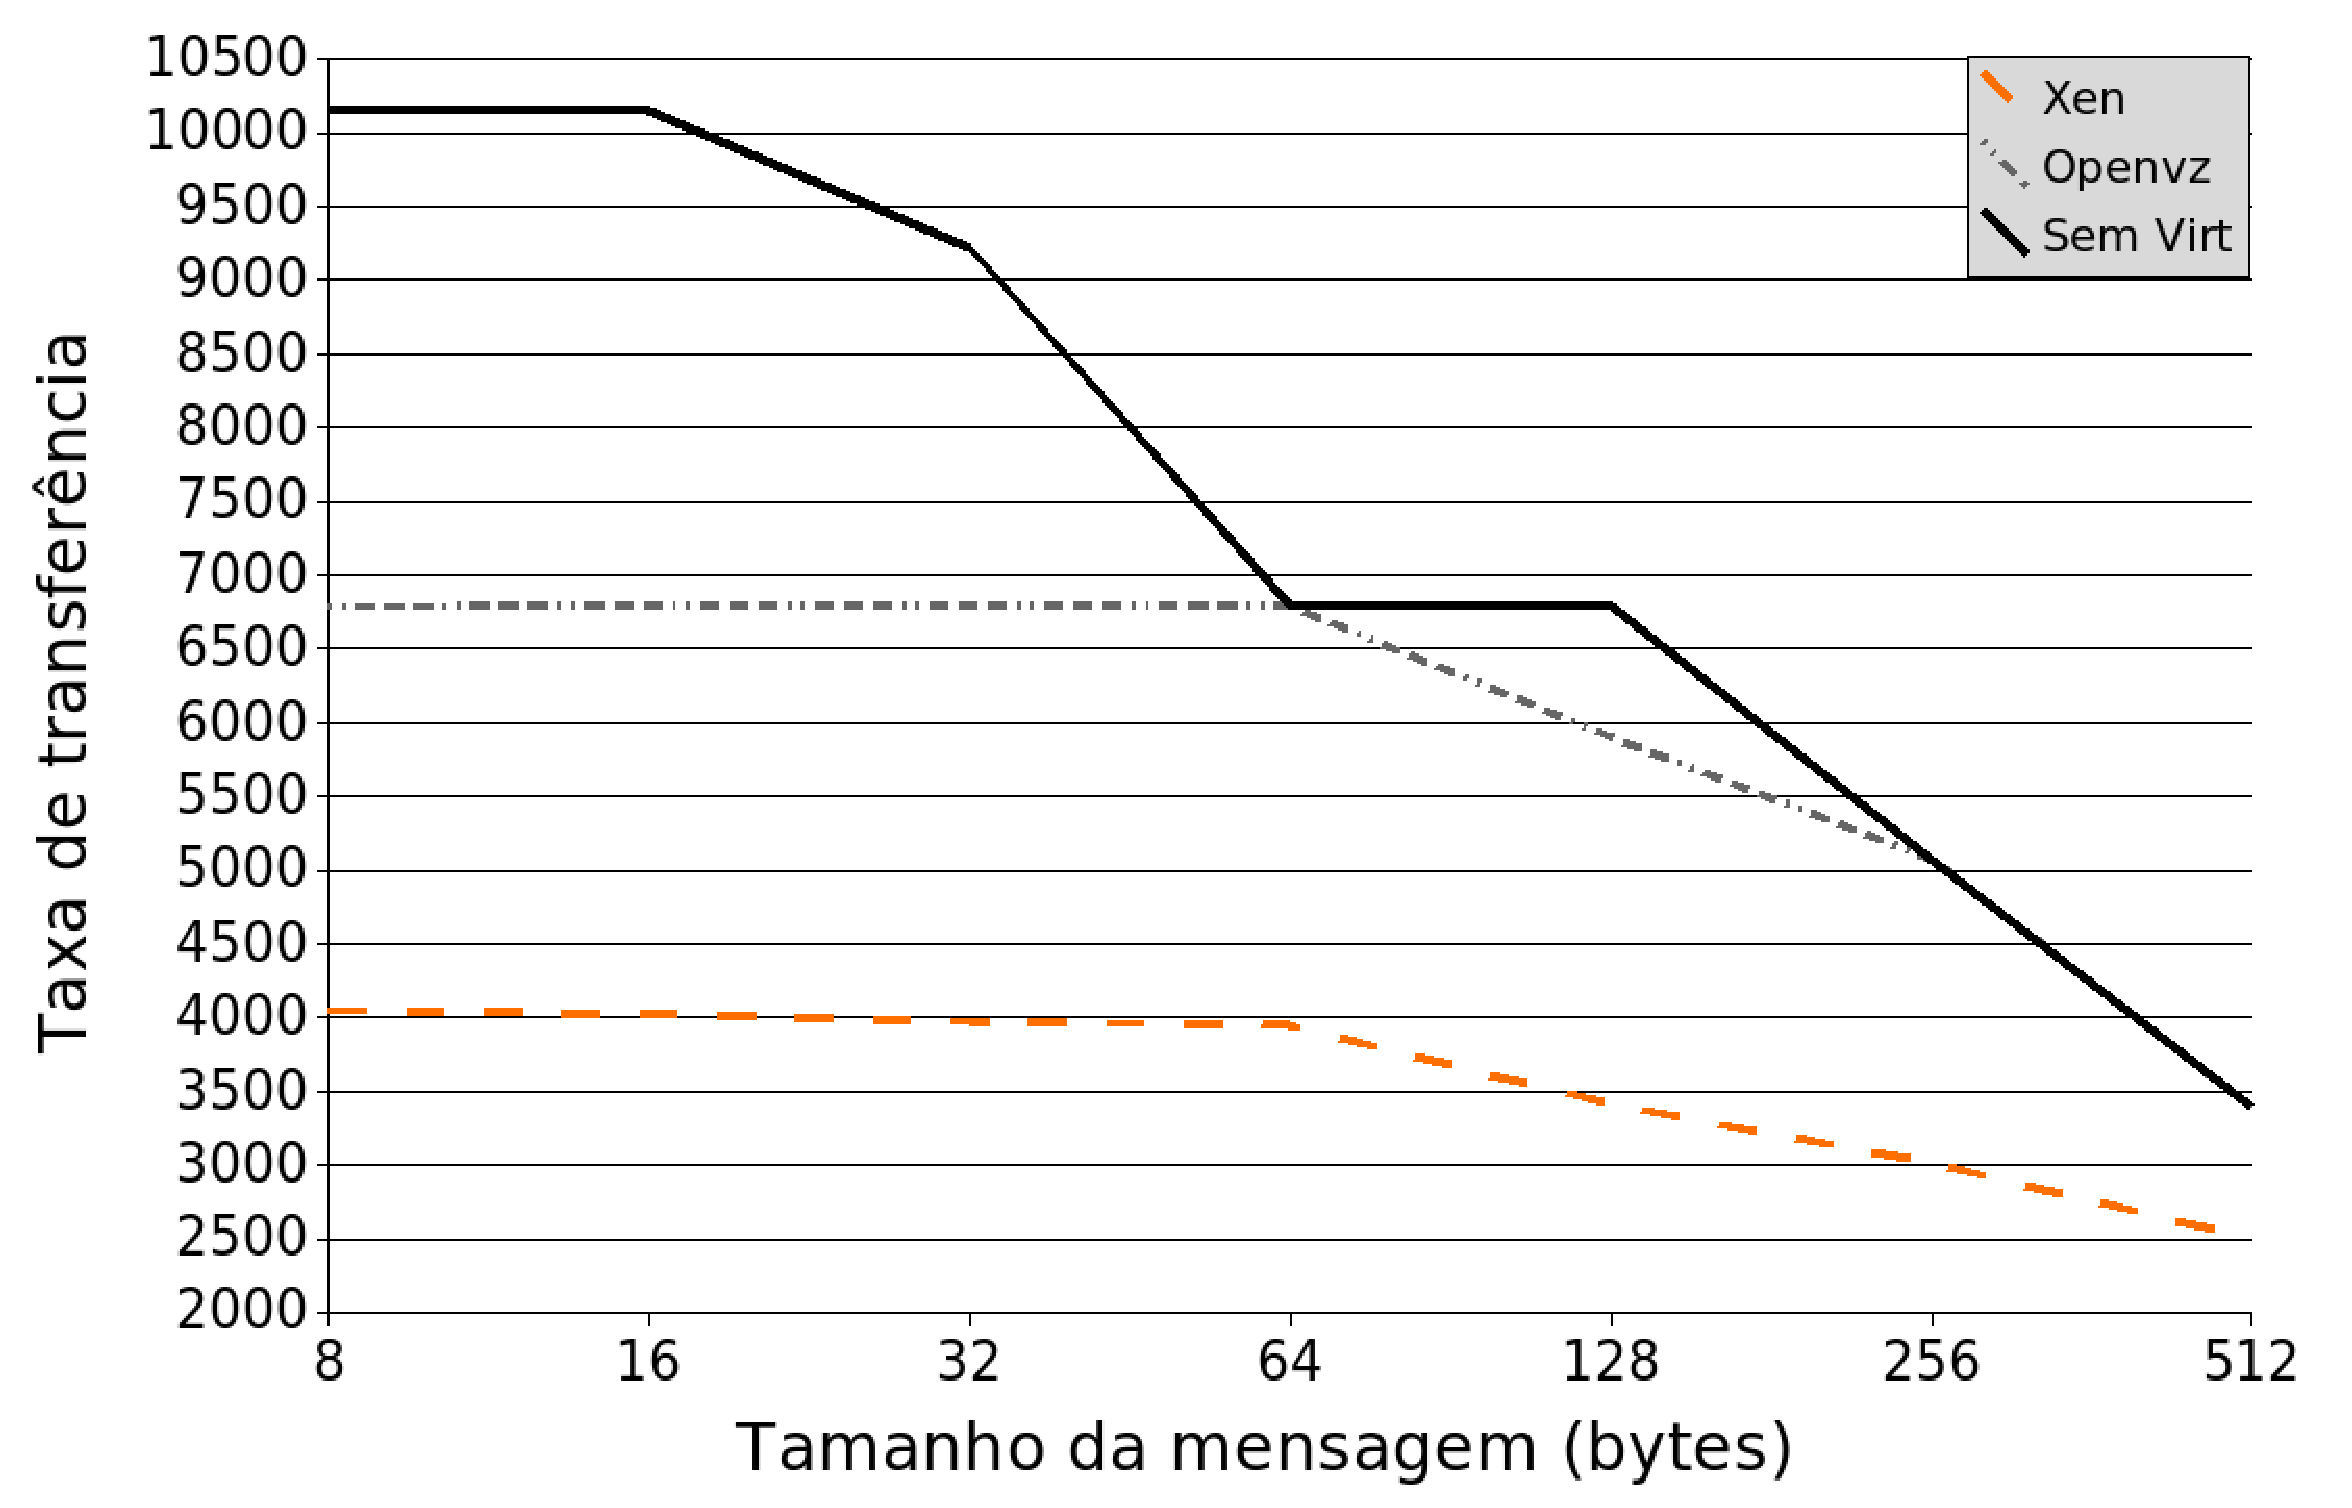
\includegraphics{figuras/udp_peq.eps}}
\caption{Taxas de transferência UDP, com mensagens  pequenas, até 512 bytes}
\label{fig:udp_peq}
\end{figure}

\begin{figure}[!htb]
\centering
\resizebox{9cm}{!}{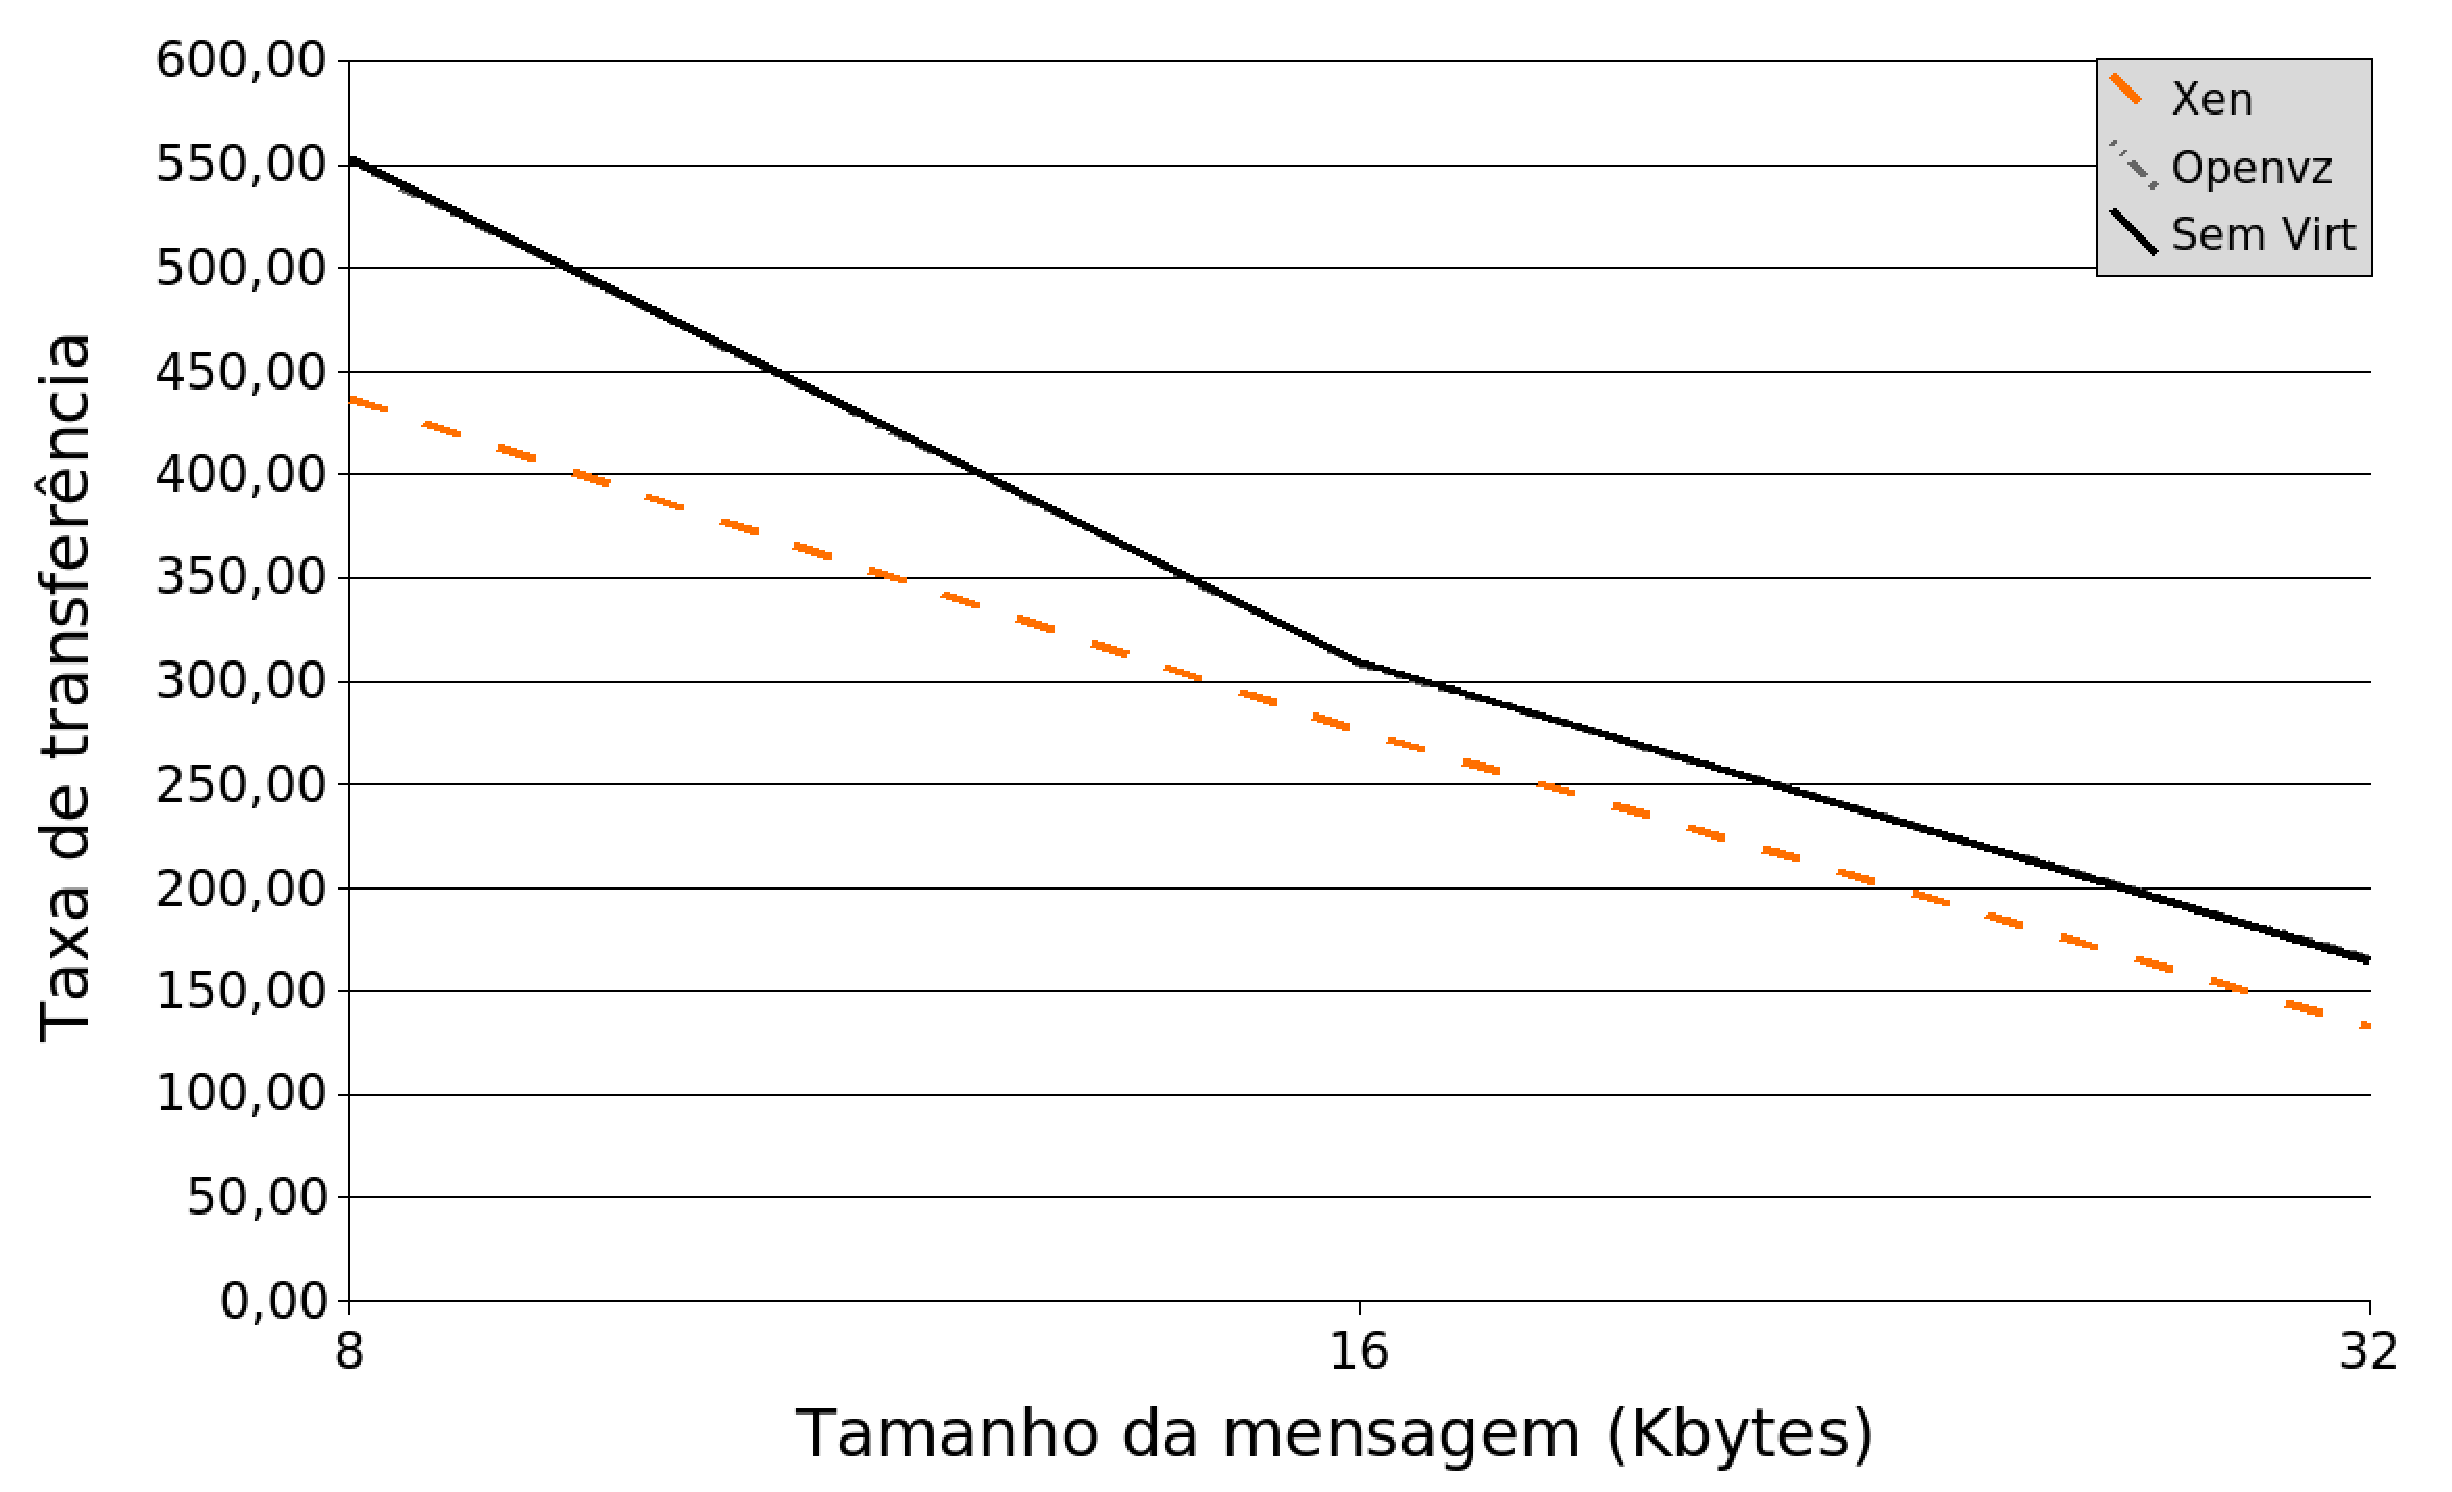
\includegraphics{figuras/udp_med.eps}}
\caption{Taxas de transferência UDP, com mensagens médias, de 8 a 32 Kbytes}
\label{fig:udp_med}
\end{figure}

%-----------------------------------------------------------------------------
\section{Considerações Finais}\label{s:fim}

Neste trabalho, analisou-se o desempenho da comunicação em uma rede entre máquinas não virtuais, virtuais usando Xen e virtuais usando OpenVZ. Observou-se que OpenVZ obteve um desempenho de rede superior ao de Xen, tanto com o protocolo TCP como com o protocolo UDP, principalmente para mensagens pequenas e médias. Também observou-se que, usando OpenVZ, o desempenho de rede é próximo àquele medido no caso sem virtualização, evidenciando uma baixa sobrecarga na rede.

Assim, dependendo da abordagem de virtualização adotada, pode-se obter resultados de desempenho significativamente diferentes. Esses resultados juntamente com a análise de outros fatores relevantes e o tipo de uso das máquinas virtuais podem prover um embasamento a administradores de sistemas no momento de selecionar uma tecnologia de virtualização a ser implantada. Além disso, a experiência obtida com este trabalho abre perspectivas para outras análises mais aprofundadas, considerando outros parâmetros que possam influenciar na comparação de desempenho entre monitores de máquinas virtuais.

%----------------------------------------------------------------------------
\bibliographystyle{sbc}
\bibliography{errc2007-xenvsopenvz}

\end{document}

%% <!-- Local IspellDict: brasileiro -->
%% <!-- Local Variables: -->
%% <!-- mode:flyspell -->
%% <!-- End: -->
